\section{Introduction}

Machine Learning (ML) is revolutionizing many fields.
It is now being used in a diverse range of domains including e-commerce, web and social media, interactive voice agents, and even in critical applications in autonomous vehicles and healthcare.
From a software systems point of view, ML can be viewed as a flexible framework for \textit{programming the unprogrammable}.
For instance, it is nearly impossible for a software developer to program an object detector that can identify different objects from an image.
But using ML and a sufficient amount of labeled training data one can \textit{learn a program} to do the same, which can even surpass human-level accuracy.

Database management systems (DBMSs) are complex software systems, that are the result of decades of research and highly-advanced engineering efforts.
They are at the core of many critical software applications and have also influenced much of the development of other popular data management systems such as NoSQL, Big Data, and Machine Learning Systems.
As the reader may be already aware, DBMSs are also full of hard unprogrammable problems. These include query optimization, physical database design optimization, buffer management, etc., which are unprogrammable either because they have interactable search spaces and/or because of the inability to predict the future. As a result, DBMS developers have to resort to using heuristics and/or scope restrictions to solve these problems. The goal of these heuristics/restrictions is not to find an optimal solution for a specific instance, but to find a solution which has a good worst-case performance on all cases.
Thus, we survey the existing landscape of using ML to program the unprogrammable in DBMSs. 

\begin{figure*}
    \centering
    \vspace{-6mm}
    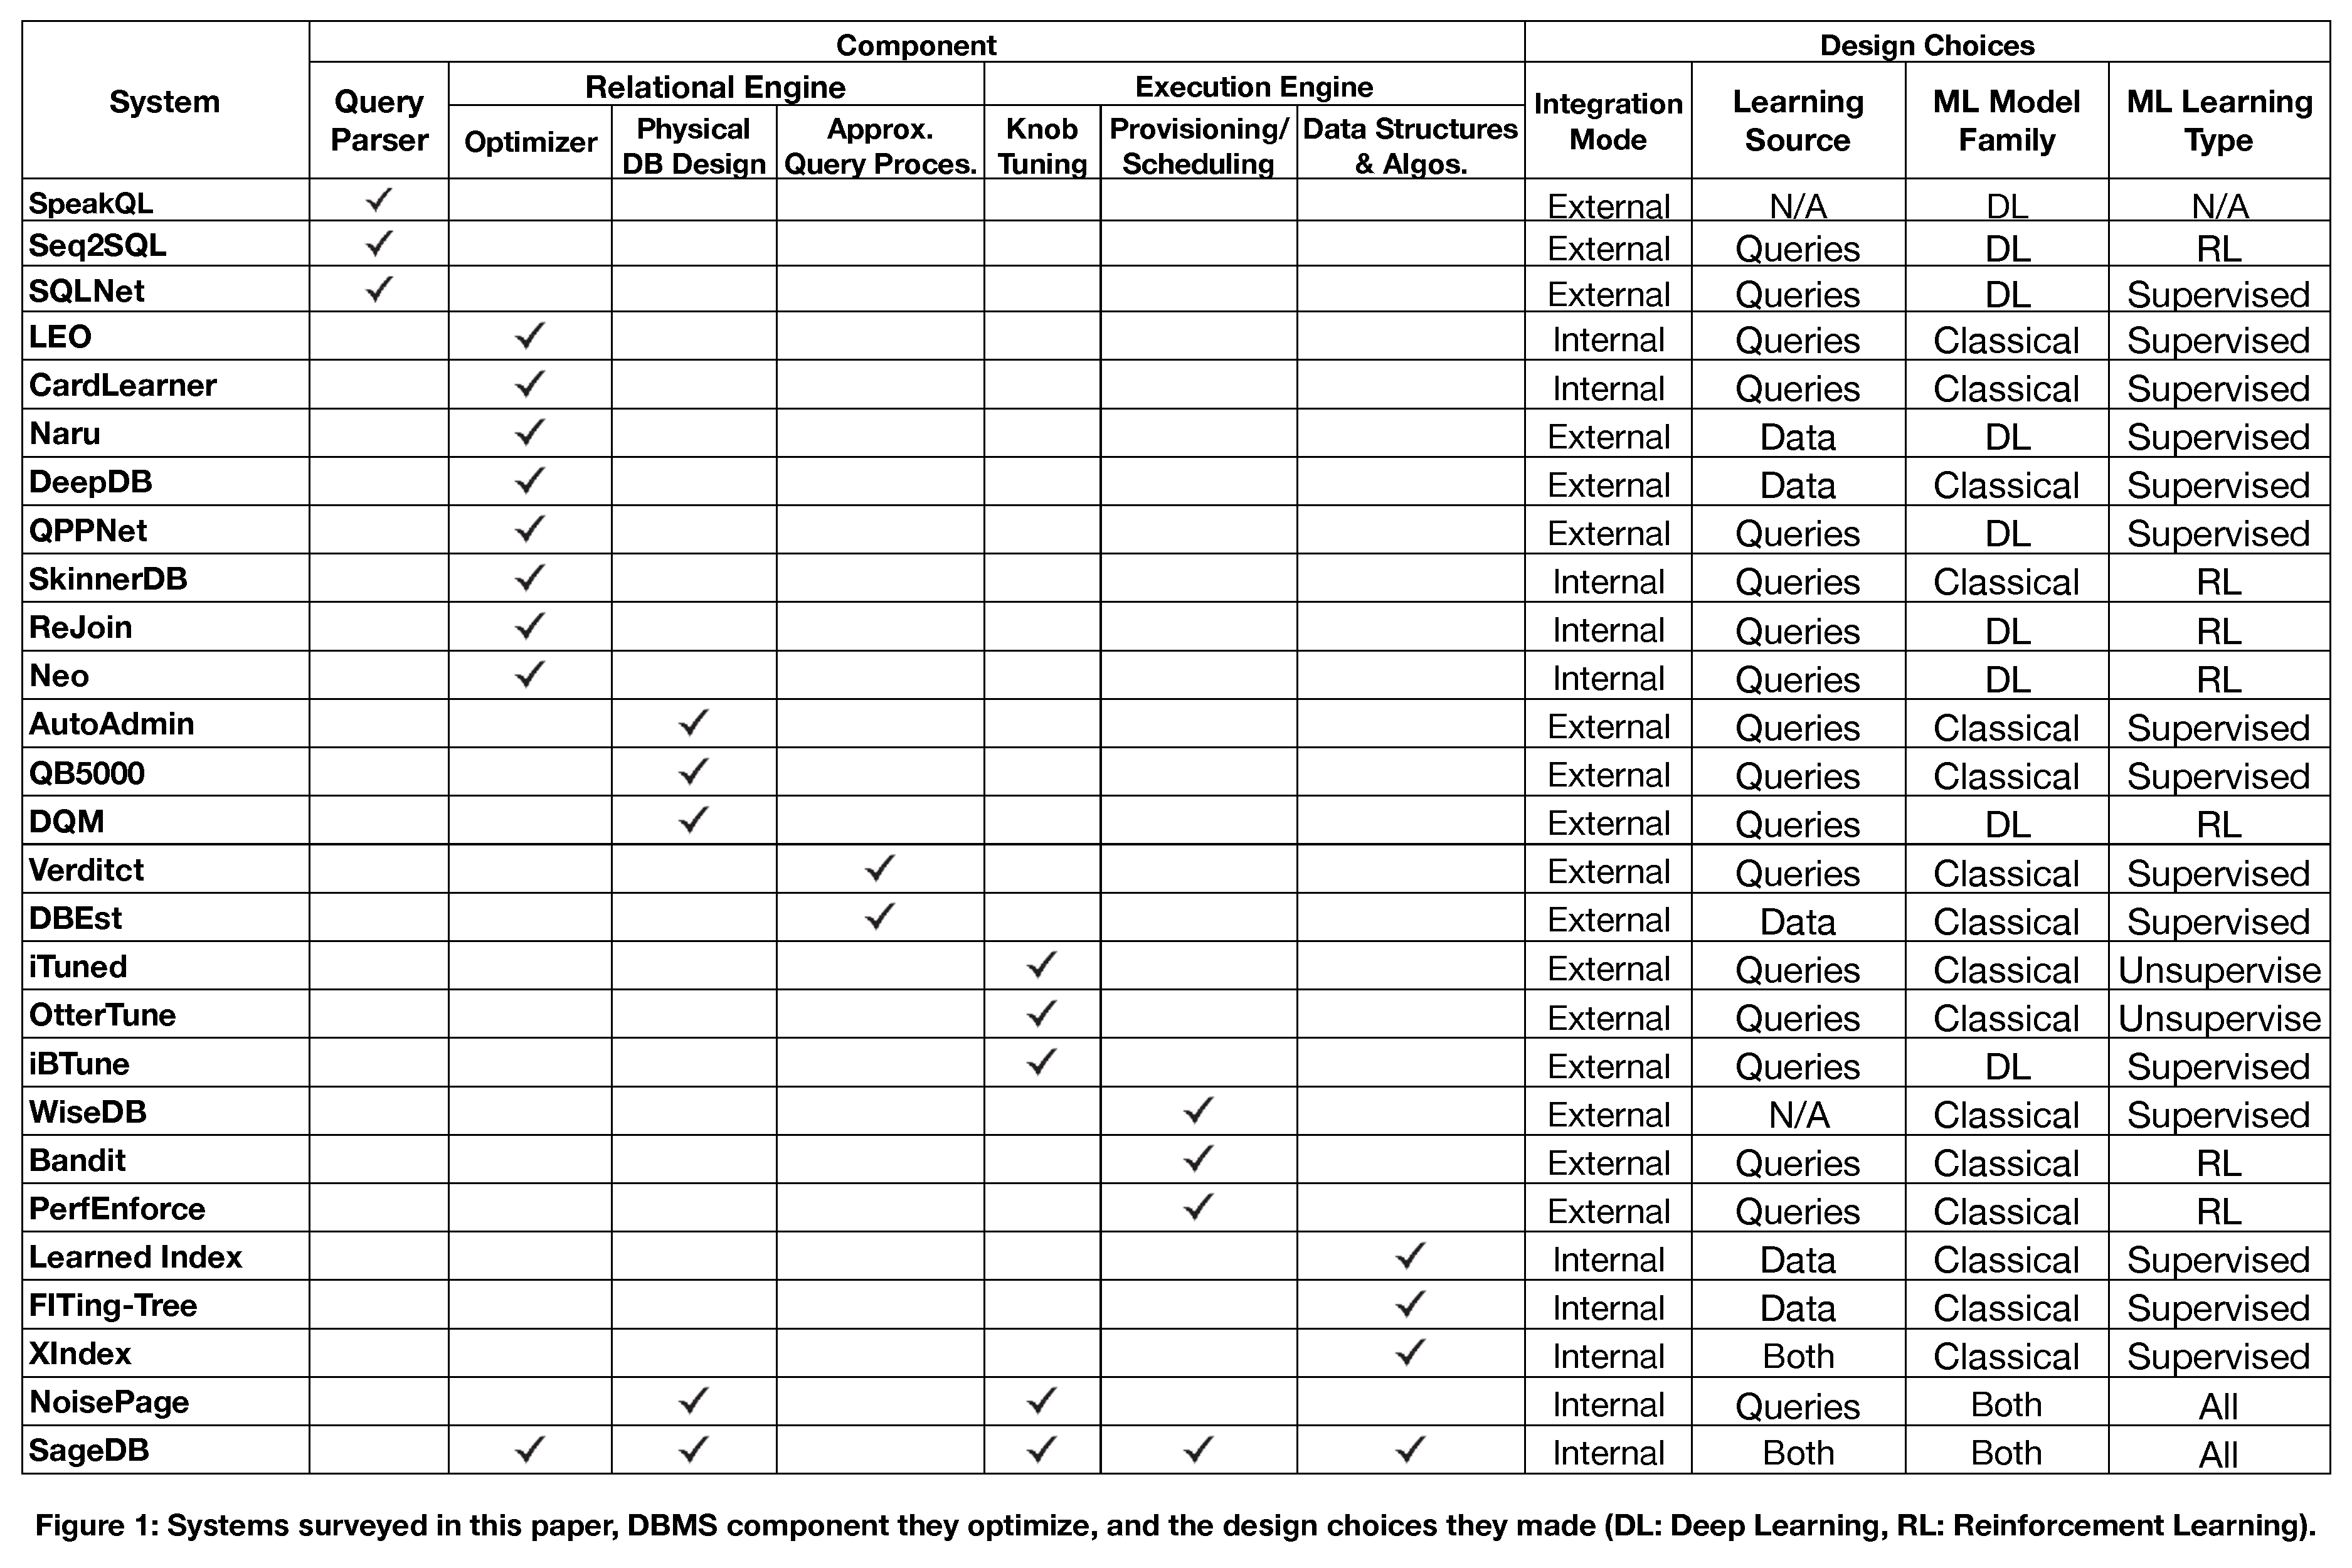
\includegraphics[height=0.85\textwidth, angle=90]{images/taxonomy.pdf}
\end{figure*}

Out of the many types of database management systems, relational database management systems (RDBMSs) remain the most widely used type.
Thus for this paper, we primarily focus on RDBMSs.
We divide the DBMS into three main sub-components: 1) Query Parser, 2) Relational Engine, and 3) Execution Engine. Some background on each of these sub-components and different ML methods is provided in Section 2.
We then identify several systems that have proposed using ML in Query Parser, Relational Engine, and Execution Engine in Section 3, 4, and 5, respectively.
In Section 6, we also identify three overarching design decisions that a DBMS developer has to make when incorporating ML into a DBMS: 1) integration mode, 2) learning source, and 3) choice of ML paradigm, and also discuss the trade-offs of available options.
A summary of where the surveyed systems fall in this taxonomy is presented in Figure 1.
While there are major accomplishments, the field is still in its infancy and many challenges remain open.
In Section 7, we identify three such open challenges: 1) improving robustness, 2) rethinking DBMS architecture, and 3) enabling transfer learning.
We give our concluding remarks in Section 8.